\documentclass[12pt,a4paper]{article}
\usepackage[T1]{fontenc}
\usepackage[a4paper]{geometry}
\usepackage[portuges,brazilian]{babel}
\usepackage[utf8]{inputenc}
\usepackage{setspace}
\usepackage{libertine}
\usepackage{graphicx}	
\usepackage{ragged2e} 
\usepackage{adjustbox}
\usepackage{float}


\begin{document} 
\begin{figure}
    \flushright
    
\includegraphics[scale=0.5]{Logo_senai.png}
\end{figure}

\title{Roteiro da apresentação sobre \emph{deep learning} aplicada a veículos autônomos}
\author{Jéssica Motta\thanks{jessicalimamotta@gmail.com. SENAI-CIMATEC. CCRoSA- Centro de Competência em Robótica e Sistemas Autônomos.}}
 

    \maketitle
    \pagenumbering{arabic}
    \singlespacing

    \section{Audiência}
    % \textbf{AUDIÊNCIA}

    \par As pessoas que irão assistir a apresentação são em sua maioria pessoas do meio acadêmico, professores, estudantes, pesquisadores e também pessoas que tenham interesse nesse assunto, que iniciaram o contato com a área de tecnologia ou possuem um profundo conhecimento da área com possibilidade de publicações neste âmbito. Pessoas que queiram aprofundar ou conhecer como são empregadas as técnicas de \emph{deep learning} em veículos autônomos, abrindo espaço para perguntas e contribuições por parte da audiência.

    \section{Contexto}
    \par A motivação de abordar este assunto encontra-se nos benefícios que o uso de \emph{Deep learning} traz quando aplicado aos veículos autônomos pois esta técnica se assemelha ao cérebro humano dando a habilidade ao carro de "pensar", ver os obstáculos e tomar decisões. Como disse Fei-Fei Li: “Se queremos máquinas para pensar, precisamos ensiná-las a ver” \cite{1}. Esta aplicação, em veículos autônomos, pode proporcionar autonomia para pessoas com deficiência física e reduzir o número de acidentes no trânsito pois boa parte deles são causados por sono, desatenção, estresse e álcool. 
    \par Além de tratar de um tema que está em evidência já que diversas empresas prometeram veículos autônomos em um curto prazo de tempo  e atualmente a maioria das iniciativas partem das universidades como por exemplo o Iara (Intelligent Autonomous Robotic Automobile) da UFES e trabalhos de conclusão como o Mini carro autônomo com deep learning \cite{2}
    
    
    % e as pessoas têm a expectativa de poder se deslocar tendo a comodidade de um veículo particular e ao mesmo tempo realizar outras atividades como assistir a um filme, ler, jogar ou falar ao celular. E por também a \emph{deep learning} ser uma das temáticas mais importantes no meio de aprendizado de máquina e redes neurais.
    \section{Seções}


    \subsection{Contar uma história}
    \par Neste momento fazer o link com o público através da identificação. Trazer a história que assim como eu muitas pessoas trabalham em cidades diferentes das quais residem e que muitas vezes fazem viagem de horas para realizarem esse trajeto, cansadas e com outras demandas como saber como a família está e resolver problemas. Trazer dados sobre o número de acidentes anuais no trânsito \textit{versus} a quantidade de acidentes causados pelos carros autônomos, já inserindo a ideia de que ter carros autônomos é algo positivo.

    % \subsection{Levantar prós do uso dos veículos autônomos}
    % \par Pontuar que a utilização destes veículos resolveria problemas no trânsito, pelo sistema apresentar uma resposta mais rápida aos estímulos e também por proporcionar autonomia para pessoas com deficiência física.
    % \par Guiar um veículo com segurança é algo que os seres humanos precisam de tempo de instrução, prática e adaptação. Dirigir exige conhecimentos prévios como: leis de trânsito, reconhecimento de objetos, noções de velocidade e distância, tomadas de decisões e definições de trajetos \cite{1}. 
    % \par Abordar que o emprego da deep learning em veículos autônomos reduziria a quantidade de acidentes já que esse tipo de \emph{machine learning} é focado em identificar objetos e realizar previsões.


    \subsection{Estrutura de um veículo autônomo}
    \par Explicar de forma resumida como é composta a estrutura de um veículo autônomo, trazendo imagens para ilustrar o que está sendo dito, nivelando que já conhece do assunto e quem não conhece. 

    \subsection{Evolução dos carros autônomos}
    \par Fazer uma linha do tempo mostrando o que foi inserido e modificado nos carros autônomos. Usar imagens para ilustrar o que será dito e facilitar a compreensão.

    \subsection{Explicar a diferença entre IA, ML e DP}
    \par Explicar as diferenças entre \emph{Inteligência artificial, machine learning e deep learning.} Esclarecer que não se trata de sinônimos. Trazer imagens e animações, como exemplificado na Figura \ref{fig:ml_dp} \cite{2}.

    \begin{figure}[H]
        \centering
        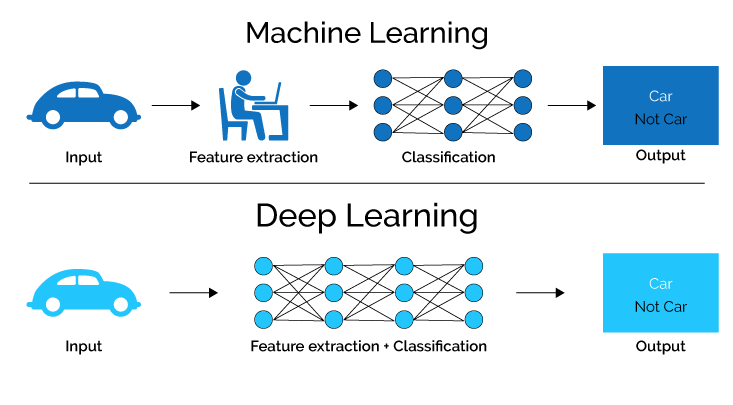
\includegraphics[scale=0.5]{ml_dp.png}
        \caption{Machine learning vs. deep learning.}
        \label{fig:ml_dp}
    \end{figure}

    \subsection{Deep learning- Um breve histórico}
    \par Abordar sobre a história da DP, falar sobre o hiato que existiu pois a DP é antiga mas não existia GPU para processamento desta rede até 2012- AlexNet.

    \subsection{Como funciona a Deep learning?}
    \par Trazer animações para explicar como funciona a \emph{deep learning} na Figura \ref{fig:dp_works} \cite{3}. Falar sobre os parâmetros de forma didática. E introduzir uma parábola para explicar melhor o funcionamento da DP.

    \begin{figure}[H]
        \centering
        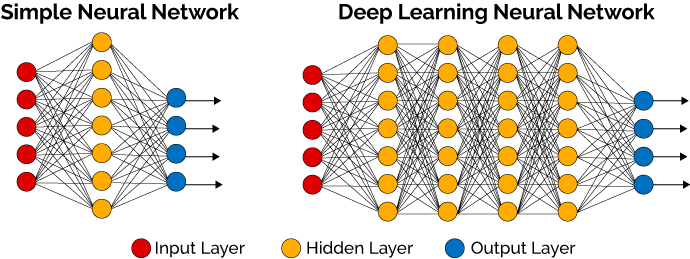
\includegraphics[scale=0.5]{dp_works.png}
        \caption{Diferença entre uma rede neural simples e a deep learning.}
        \label{fig:dp_works}
    \end{figure}
    


    \subsection{Como ela está aplicada aos veículos autônomos?}
    \par E como a \emph{deep learning} está inserida nos veículos autônomos. Tratar de reconhecimento de objetos e métodos de identificação. Falar sobre classificação de imagens, classificação e localização, detecção de objetos e segmentação de instâncias, pontuando as diferenças entre elas e qual a melhor a ser empregada em veículos autônomos com \emph{deep learning}.


    % \subsection{Citar empresas que estão construindo veículos autônomos}
    % \par Fazer um comparativo do que já vem sendo feito nos últimos anos pelas empresas, tais como Tesla, Uber, Google etc. Quais os avanços que conseguiram e quais as perspectivas futuras destas empresas focando em \emph{deep learning}.

    \subsection{Conclusão}
    \par Encerrar falando sobre a visão computacional e \emph{deep learning} nos veículos autônomos, e o quanto impacta na qualidade da identificação, fazendo uma revisão do que foi visto anteriormente nos outros tópicos, a retomada é importante para reforçar o que foi visto.

    

    \section{Tempo}
    \par Haverá 20 min destinados para apresentação do conteúdo, onde os slides servirão de suporte para o assunto exposto, dedicando entre 1 min e 1:30 min para cada slide.  
    
    \section{Perfil}
    \par A intenção é de passar um perfil que possui certo conhecimento sobre o assunto exposto, falando pausadamente e no tom que as pessoas consigam acompanhar, e que ainda assim tem também interesse em aprender com o público. Para fazer isso a apresentação será estudada nos mínimos detalhes e ensaiada, refletir sobre o que será falado em cada slide e as possibilidades de contestação e pesquisa para responder o máximo de perguntas que surgirem.


     
    \begin{thebibliography}{BIBLIOGRAFIA}

        \bibitem{1} https://www.startse.com/noticia/startups/mobtech/deep-learning-o-cerebro-dos-carros-autonomos
        
        \bibitem{2} MANICA, Bruno et al. Mini Carro Autônomo com Deep Learning. 2019.

        \bibitem{3} DELAI, Riccardo L.; COELHO, Alessandra Dutra. \textbf{DESENVOLVIMENTO DE VEÍCULO AUTÔNOMO-INTELIGÊNCIA CENTRAL E ORIENTAÇÃO POR CÂMERAS.}
        \bibitem{4} http://www2.decom.ufop.br/imobilis/inteligencia-artificial-e-deep-learning/

        
    
    \end{thebibliography}

    % https://medium.com/brasil-ai/como-funcionam-os-carros-aut%C3%B4nomos-parte-1-sensoriamento-e-vis%C3%A3o-computacional-ae25d17c66a1

    % https://tecnoblog.net/286916/tesla-carros-autonomos-robotaxis-fsd/


    % https://www.google.com/search?q=gruta+de+bom+jesus+da+lapa&sxsrf=ALeKk02m7o7USbENUMebHaJ5b4V_fX5UWA:1595337552918&source=lnms&tbm=isch&sa=X&ved=2ahUKEwicx43Bt97qAhUUF7kGHdn8D3AQ_AUoAXoECA8QAw&biw=1920&bih=928

    % http://ecmetrics.com/pt/ai-machine-learning-deep-learning/

    % http://datascienceacademy.com.br/blog/segmentacao-de-imagens-medicas-com-deep-learning/


\end{document}